\documentclass[]{beamer}

\usepackage[utf8x]{inputenc}


% opciones para la presentacion
\usetheme{Warsaw}
% \usetheme{classic}

% multifiguras
% \usepackage{graphicx}
\usepackage{subcaption}


%datos de la presentacion
\title{Seguimiento de objetos en secuencias de imágenes RGB-D}
\subtitle{Tesis de licenciatura}
\institute{Facultad de Ciencias Exactas y Naturales}
\date[18/03/15]{Miércoles 18 de Marzo de 2015}
\author[Mariano Bianchi]{Mariano Bianchi}


\begin{document}

\maketitle
%--- Next Frame ---%



%%%%%%%%%%%%%%%%%%%%%%%%%%
%%%%%%%%%%%%%%%%%%%%%%%%%%
\section{Introducción}
\begin{frame}[t]{Si nos organizamos...}
    \tableofcontents
    % comentar como va a estar organizada la charla
\end{frame}
%--- Next Frame ---%

\subsection{Motivación}
\begin{frame}{Aplicaciones} % si pongo la opcion [t] el texto empieza desde arriba
    % Permite generar estadísitcas deportivas midiendo la distancia recorrida por
    % jugadores de futbol, tiros al arco, goles, faltas realizadas, etc
    \begin{figure}[t]
        \centering
        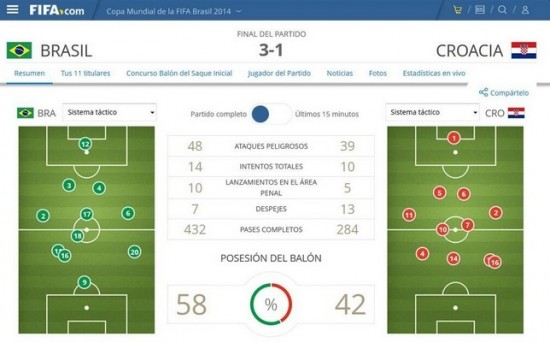
\includegraphics[scale=0.5]{img/estadistica.jpg}
    \end{figure}
\end{frame}

\begin{frame}{Aplicaciones}
    % Permite que un robot sepa de que manera tomar un objeto y usarlo como
    % herramienta de trabajo
    \begin{figure}[t]
        \centering
        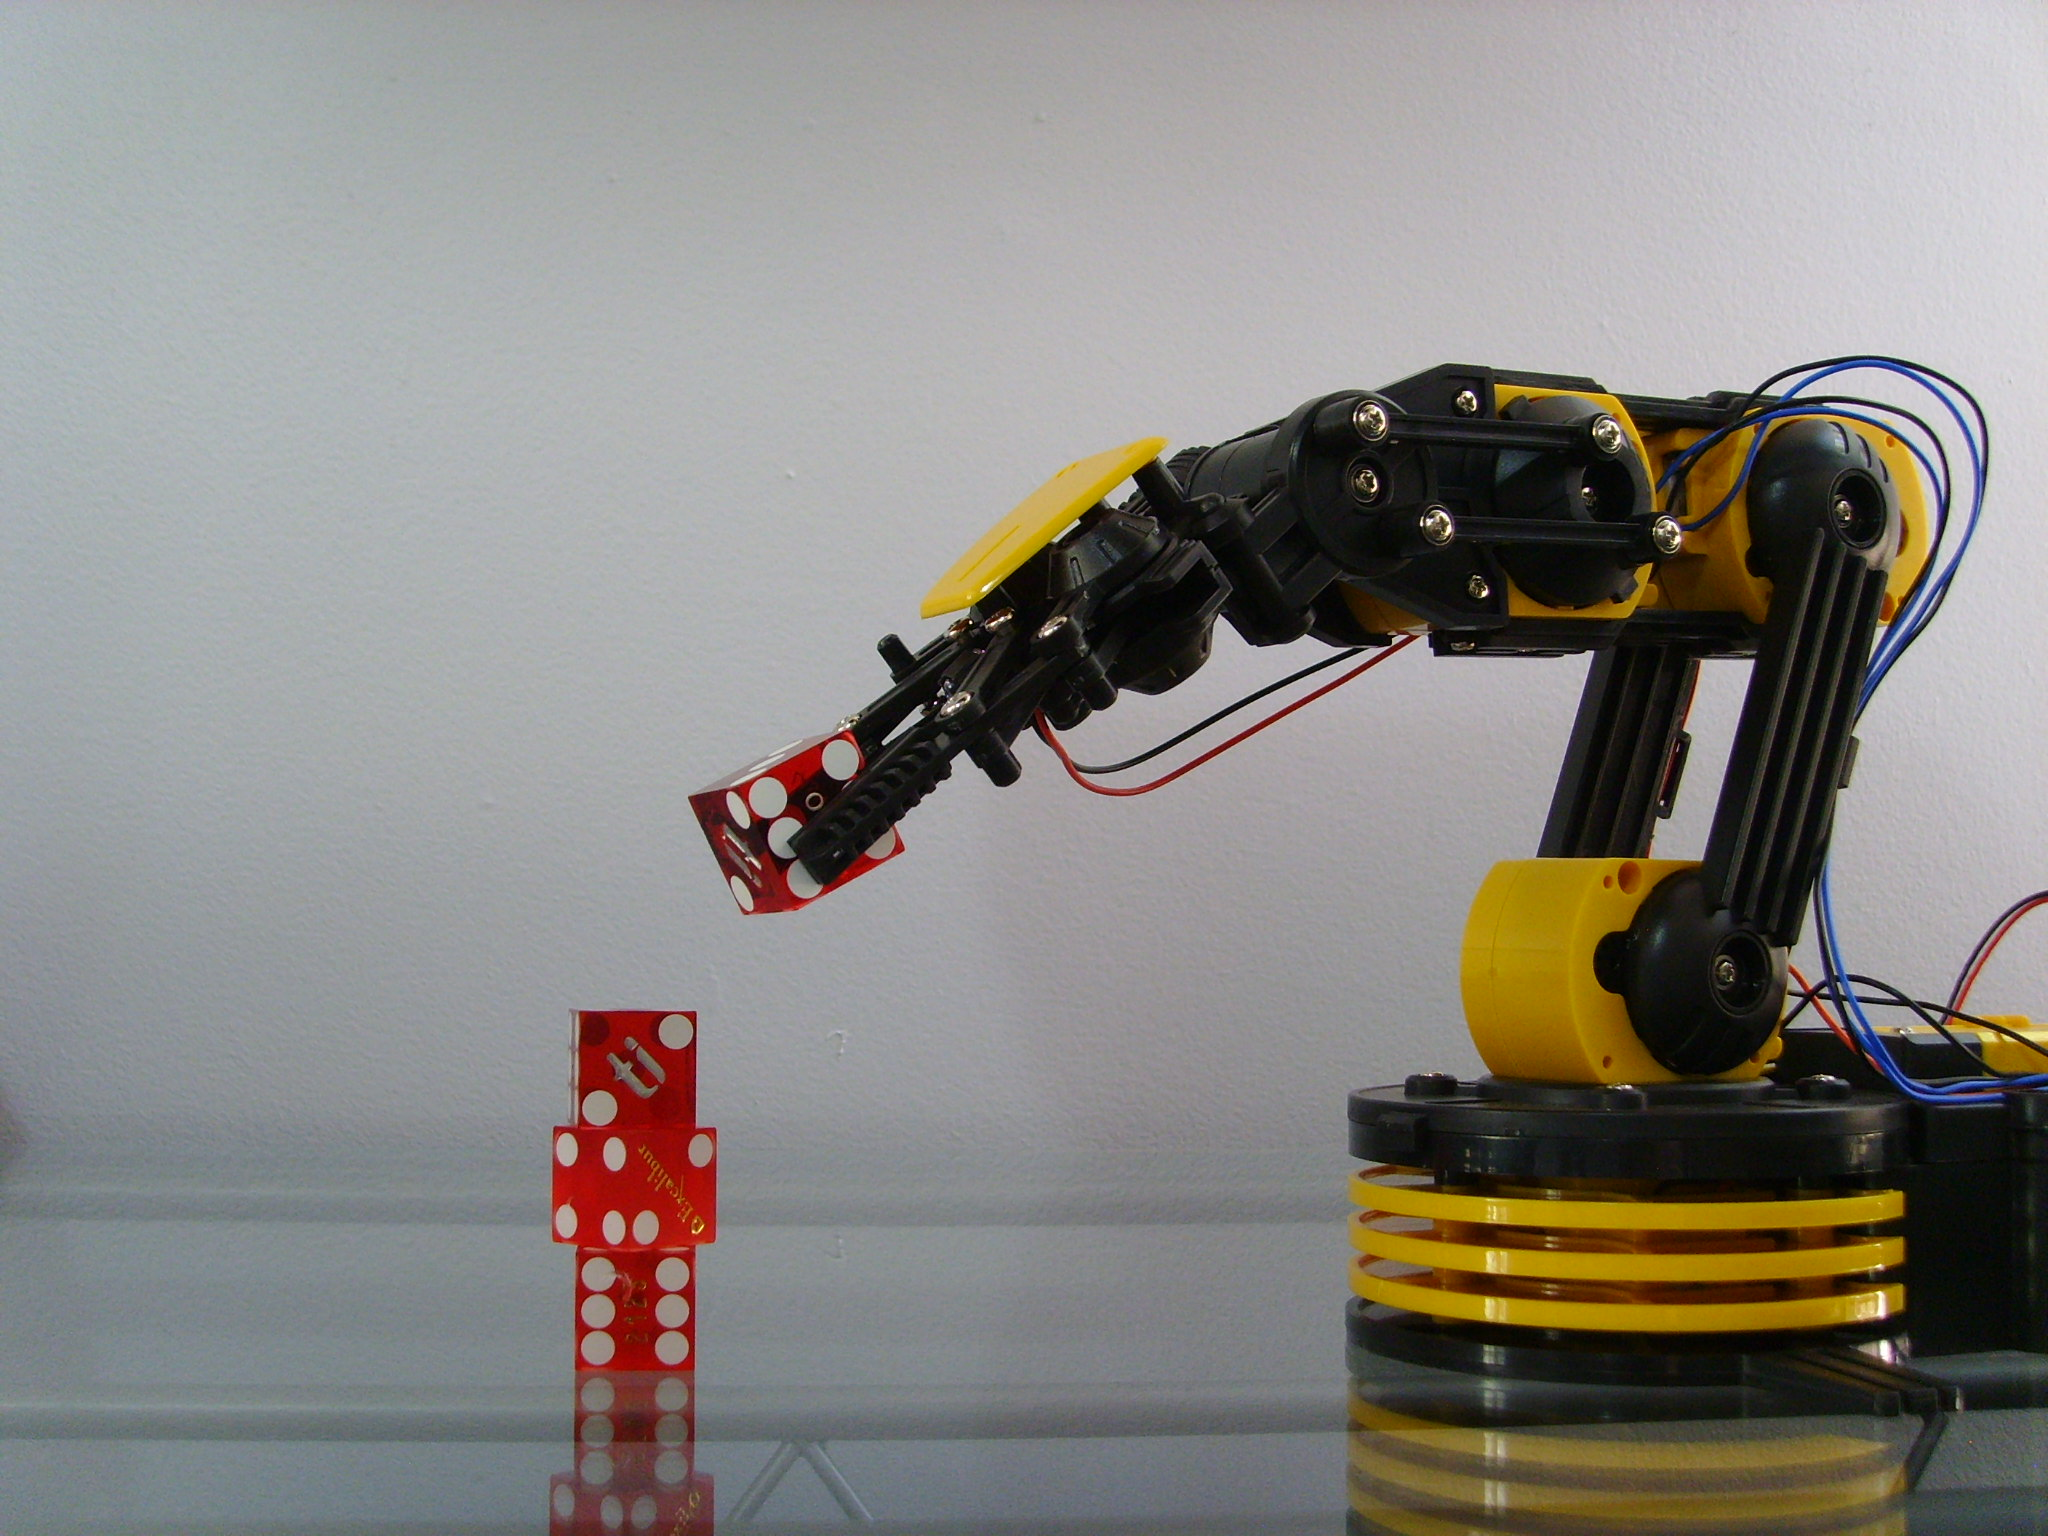
\includegraphics[scale=0.12]{img/robot.jpg}
    \end{figure}
\end{frame}

\subsection{Vamos por partes... del título}
\begin{frame}{Seguimiento}
    % El comportamiento esperado de un método de seguimiento es obtener para
    % cada imagen de una secuencia de imágenes o video la ubicación de un
    % objeto en algún eje de coordenadas elegido
    IMAGEN DE UN FRAME CON EL OBJETO EN UN RECUADRO Y MARCANDO LAS COORDENADAS
    DE LOS PIXELES QUE LO DESCRIBEN
\end{frame}
%--- Next Frame ---%



\begin{frame}{Objetos}
    \begin{figure}[t]
        \centering
        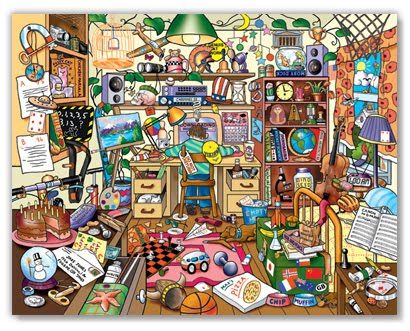
\includegraphics[scale=0.6]{img/escena_con_objetos.jpg}
    \end{figure}
\end{frame}
%--- Next Frame ---%



\begin{frame}{Secuencia de imágenes}
    % Puede ser un video, una ráfaga de imágenes tomada con una cámara de fotos
    \begin{figure}[t]
        \centering
        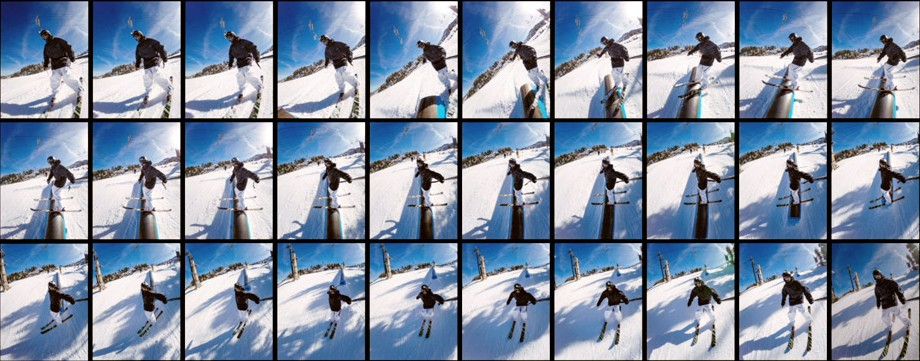
\includegraphics[scale=0.35]{img/rafaga_1.jpg}
    \end{figure}
\end{frame}
%--- Next Frame ---%



\begin{frame}{El RGB de las imágenes RGB-D}
    % Una imagen RGB-D está compuesta por dos partes. Una de ellas es una
    % imagen RGB
    % Las imágenes RGB son las más comunes y que todos conocen. Es simplemente
    % una fotografía. RGB significa Red Green Blue, que son los colores
    % primarios lumínicos (en el dominio de la luz), es decir, que el resto de los colores puede definirse
    % con una combinación de estos tres colores
    \begin{block}{}
        PEGAR UNA IMAGEN RGB CUALQUIERA
    \end{block}
\end{frame}
%--- Next Frame ---%

\begin{frame}{El D de las imágenes RGB-D}
    % Un sensor RGB-D cuenta con una cámara tipo webcam que otorga imagenes RGB,
    % un proyector infrarrojo y una cámara infrarroja. El proyector dibuja un patrón
    % conocido en la escena, que al ser infrarrojo es invisible al ojo humano.
    % Luego la cámara infrarroja captura ese patrón proyectado y utilizando algoritmos
    % de luz estructurada junto con las distancias conocidas entre la cámara y proyector
    % infrarrojo se puede obtener la profundidad para cada pixel de la escena.
    \begin{block}{}
        MOSTRAR SENSOR RGB-D, contar como funciona y mostrar con el pcl\_viewer una nube de puntos y una imagen RGB-D
    \end{block}
\end{frame}
%--- Next Frame ---%


\begin{frame}[t]{Sistema de seguimiento}
    % Un sistema de seguimiento tiene al menos 3 etapas bien definidas
    \begin{figure}[t]
        \centering
        \vspace{-13pt}
        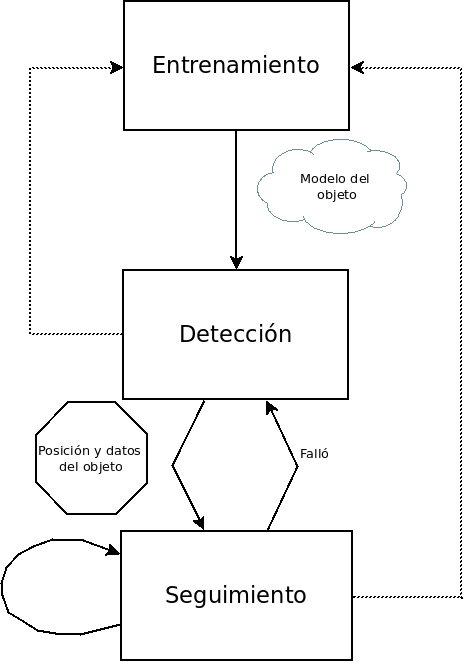
\includegraphics[scale=0.3]{img/esquema_seguimiento.png}
    \end{figure}
\end{frame}
%--- Next Frame ---%


\subsection{Objetivos}
\begin{frame}[t]{Objetivos}
    \begin{block}{Sistema RGB-D}
        Implementar, estudiar y evaluar un sistema de seguimiento RGB-D, enfocándonos especialmente en la etapa de seguimiento
    \end{block}
    \begin{block}{Análisis}
        Comparar métodos de seguimiento en RGB y en profundidad y comprender en que casos es conveniente usar uno u otro método, cuándo y de qué manera combinarlos
    \end{block}
    % TODO: preguntar por esto
    \begin{block}{Aportes???}
        Obtener resultados que puedan ser utilizados como base de comparación frente a otros sistemas de seguimiento
    \end{block}
\end{frame}
%--- Next Frame ---%



%%%%%%%%%%%%%%%%%%%%%%%%%%
%%%%%%%%%%%%%%%%%%%%%%%%%%
\section{Desarrollo}
% TODO: cambiarle el titulo al frame por algo mejor
\begin{frame}{Distintos esquemas para el mismo problema????}
    % IDEA DE ESTE SLIDE: motivaciones, por que la separacion de los metodos,
    % comparar metodos rgb y d

    % Partiendo del esquema antes visto como base de nuestro sistema de seguimiento
    % nos propusimos desarrollar un sistema de seguimiento RGB, uno en profundidad
    % y luego utilizar lo mejor de cada uno para crear un sistema RGB-D que
    % combine lo mejor de cada uno
    % El motivo por el cual desarrollamos 2 sistemas por separado es para poder
    % cuantificar las diferencias entre usar alguno de esos sistemas por separado
    % o uno que los combine y decidir cual se comporta mejor en general o en cada
    % situacion en particular
    \begin{itemize}
        \item Sistema RGB completo y funcional
        \item Sistema en profundidad completo y funcional
        \item Combinarlos de la mejor manera posible
        \item Obtener resultados comparables frente a métodos existentes
    \end{itemize}

\end{frame}
%--- Next Frame ---%

\subsection{Sistema RGB}
\begin{frame}[t]{Detección RGB}

    En esta etapa usamos un método llamado \textit{template matching}. Para utilizarlo necesitamos:
    \begin{itemize}
        \item \textit{templates}: Una o más imágenes del objeto a detectar tomadas de diferentes ángulos
        \item \textit{escena}: Un frame de un video o imagen en donde se desea ubicar el objeto
        \item Opcionalmente podemos utilizar máscaras que segmenten al objeto en cada template.
    \end{itemize}
\end{frame}
%--- Next Frame ---%

\begin{frame}[t]{Detección RGB}

    PONER ESTAS IMAGENES
    \begin{enumerate}
        \item Un template entero
        \item Un template segmentado
        \item Una escena
    \end{enumerate}
\end{frame}
%--- Next Frame ---%



\begin{frame}[t]{Detección RGB}
    \begin{block}{Pasos del algoritmo de template matching}
        Para cada template proveniente del entrenamiento y para cada pixel de la escena, seguir estos pasos:
        \begin{enumerate}
            \item Tomar un rectángulo de la escena del tamaño del template cuya esquina superior izquierda sea el pixel actual
            \item Compararlo con el template (ejemplo: diferencia cuadrática pixel por pixel)
            \item Si la comparación está por debajo de un umbral predefinido y es el mejor valor encontrado, guardar la ubicación del pixel
        \end{enumerate}
        Una vez recorrida toda la imagen, se devuelve la ubicación del ``mejor recuadro''. Si no se encontró ninguno por debajo del umbral, se indica que no se encontró el objeto en la imagen.
    \end{block}
\end{frame}
%--- Next Frame ---%


\begin{frame}[t]{Entrenamiento RGB}
    Como el algoritmo de detección elegido es \textit{template matching}, esta etapa consta simplemente de obtener distintos templates del objeto que se desea seguir, tratando de cubrir las distintas ``caras'' del objeto desde varias alturas. Por ejemplo:
    \begin{block}{}
        PONER UN PAR DE TEMPLATES
    \end{block}
\end{frame}
%--- Next Frame ---%


\begin{frame}[t]{Seguimiento RGB}
    Tomando la ubicación del objeto en el frame anterior, se explora en un área cercana (mucho menor que el área de la escena) de manera similar a la de \textit{template matching} en búsqueda del objeto deseado. Para cada recuadro explorado se siguen estos pasos:
    \begin{enumerate}
        \item Calcular histograma del recuadro
        \item Calcular histograma del recuadro del frame anterior
        \item Calcular histograma del último template ``matcheado''
        \item Comparar los histogramas 1-2 y 1-3
        \item Si ambas comparaciones están por debajo de sus respectivos umbrales y son las mejores, se guarda la ubicación del recuadro (esq. superior izquierda)
    \end{enumerate}
    Si se guardó una ubicación, se la devuelve como resultado. Si no, se indica que no se encontró el objeto y se vuelve a la etapa de detección
\end{frame}
%--- Next Frame ---%



\subsection{Sistema en profundidad}
\begin{frame}[t]{Detección en profundidad}

    Para esta etapa vamos a usar dos métodos de alineación de nubes de puntos y combinarlos. Para usarlos necesitamos:
    \begin{itemize}
        \item \textit{vista del objeto}: Una nube de puntos del objeto parcial o completa (similar al concepto de template en RGB)
        \item \textit{escena}: Una nube de puntos de la escena donde se desea encontrar al objeto
    \end{itemize}
\end{frame}
%--- Next Frame ---%

\begin{frame}[t]{Detección en profundidad - Método 1}
    El método se llama Iterative Closest Point (ICP)
    \begin{block}{Algoritmo ICP}
        Dadas dos nubes de puntos A y B, se siguen los siguientes pasos hasta que alguna condición de corte se cumpla:
        \begin{enumerate}
            \item Se calculan los ``puntos más cercanos'' entre A y B
            \item Se calcula una transformación que una los puntos cercanos de A en B
            \item Se aplica la transformación sobre A
        \end{enumerate}
        Al terminar se devuelve la transformación T proveniente de aplicar todas las transformaciones parciales junto con el error cuadrático medio entre los puntos más cercanos de T(A) y B
    \end{block}
\end{frame}
%--- Next Frame ---%



\begin{frame}[t]{Detección en profundidad - Método 2}
    % Decir que los descriptores proveen una forma de representar caracteristicas especiales
    % en una imagen, como puede ser una forma, color, textura, movimiento, etc
    El método usado es una variante de un esquema RANSAC
    \begin{block}{RANSAC}
        Dadas dos nubes de puntos A y B, se calculan sus descriptores (features) y se siguen estos pasos:
        \begin{enumerate}
            \item Tomar N descriptores random de A
            \item Encontrar sus correspondencias en B
            \item Descartar si los poligonos resultantes no son isométricos
            \item Si lo son, estimar una transformación entre los descriptores
            \item Transformar y calcular error cuarático medio
            \item Almacenar transformación si tiene el menor error hasta ahora
        \end{enumerate}
        Al terminar se devuelve la mejor transformación T encontrada y el error cuadrático medio entre los puntos más cercanos de T(A) y B
    \end{block}
\end{frame}
%--- Next Frame ---%


\begin{frame}[t]{Detección en profundidad - Combinación}
    % Dado que ICP es sensible a outliers y no así RANSAC, utilizamos como método inicial en la detección a RANSAC y refinamos el resultado usando ICP.
    El método final comienza con una nube de puntos del objeto O y otra de la escena S. Se segmenta la escena de manera similar a \textit{template matching} y para cada segmento se siguen estos pasos:
    \begin{itemize}
        \item Aplicar RANSAC entre O y S
        \item Si no es exitoso, se continua con el siguiente segmento
        \item Si fue exitoso, aplicar ICP entre RANSAC(O) y S
        \item Si ICP fue exitoso, se almacena el resultado y se sigue con otro segmento
    \end{itemize}
    Si se almacenó algun segmento, se filtran los puntos de la escena correspondientes al objeto en ese segmento, se obtiene su ubicación en coordenadas RGB y se pasa al siguiente frame
\end{frame}
%--- Next Frame ---%


\begin{frame}[t]{Entrenamiento en profundidad}
    Como el algoritmo de detección elegido es \textit{template matching}, esta etapa consta simplemente de obtener distintos templates del objeto que se desea seguir, tratando de cubrir las distintas ``caras'' del objeto desde varias alturas. Por ejemplo:
    \begin{block}{}
        PONER UN PAR DE TEMPLATES
    \end{block}
\end{frame}
%--- Next Frame ---%


\begin{frame}[t]{Seguimiento en profundidad}
    Tomando la nube de puntos del objeto segmentado en el frame anterior y la nube de puntos de la escena en el frame actual, se siguen estos pasos:
    \begin{enumerate}
        \item Se filtran los puntos de la escena cercanos a la ubicación del objeto en el frame anterior
        \item Se aplica ICP entre el objeto y los puntos filtrados de la escena
    \end{enumerate}
    Si ICP fue exitoso, se devuelve la posición del objeto y se continua en el siguiente frame. Si falla, se vuelve a la etapa de detección sobre el mismo frame.
\end{frame}
%--- Next Frame ---%


\subsection{Sistema RGB-D}
\begin{frame}[t]{Sistema RGB-D}
    \begin{block}{Entrenamiento}
        Se unen los entrenamientos de RGB y profundidad
    \end{block}
    \begin{block}{Detección}
        Se utiliza primero la detección RGB y si es exitoso se transforman estos datos para utilizarlos con la detección en profundidad. Una detección RGB-D es exitosa siempre que lo sean ambas detecciones por separado.
    \end{block}
    \begin{block}{Seguimiento}
        Primero se aplica el seguimiento en profundidad. Si es exitoso se intenta mejorar con el seguimiento en RGB, partiendo del resultado en profundidad. Un seguimiento RGB-D es exitoso si el seguimiento en profundidad es exitoso. La parte RGB se usa solo para refinar el resultado.
    \end{block}
\end{frame}
%--- Next Frame ---%


%%%%%%%%%%%%%%%%%%%%%%%%%%
%%%%%%%%%%%%%%%%%%%%%%%%%%
\section{Resultados}
\subsection{Base de datos}
\begin{frame}{Base de datos}
    % Para poder cuantificar que tan bien funcionaron los métodos y compararlos
    % entre si utilizamos una BD de objetos y escenas de donde obtuvimos
    % información de ground truth (verdad absoluta)
    % La base tiene por un lado objetos, ordenados en diferentes categorías
    % y con distintas instancias por categoría. Por ejemplo: 5 tazas distintas
    % para la categoría tazas, 4 gorras en la categoría gorras
    % Para cada objeto tiene grabadas 3 escenas desde distintas alturas en donde
    % se filma al objeto girando sobre una base giratoria, se toman imagenes
    % cada 3 grados, se las segmenta tanto en RGB como en profundidad (nube de
    % puntos). Suman una totalidad de 300 obj
    % Además cuenta con 8 escenas en las cuales aparecen algunos de los objetos
    % de la base. Las escenas están anotadas frame por frame indicando la
    % ubicación del objeto o de los objetos en ese frame
    \begin{columns}[t]
        \begin{column}{5cm}
            \begin{itemize}
                \item 300 objetos de uso diario
                \item 51 categorías
                \item Segmentados en RGB y en profundidad
            \end{itemize}

            \begin{figure}
                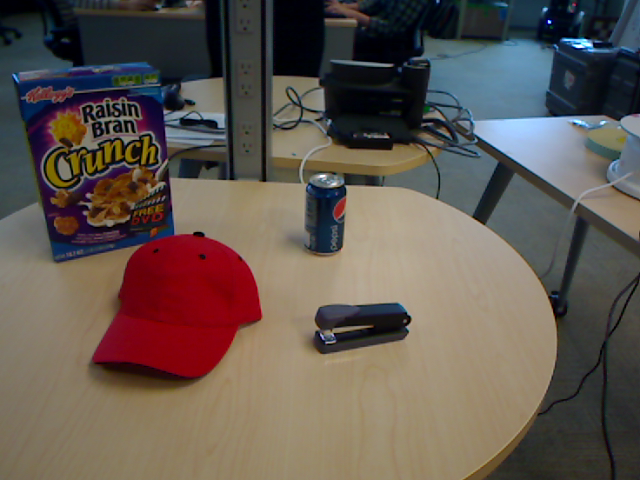
\includegraphics[width=0.8\textwidth]{img/base/scene.png}
            \end{figure}

        \end{column}
        \begin{column}{5cm}
            \begin{figure}
            	\centering
            	\begin{subfigure}{1.2cm}
            		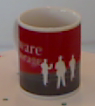
\includegraphics[width=\textwidth]{img/base/1.png}
            	\end{subfigure}
            	\begin{subfigure}{1.2cm}
            		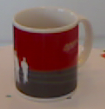
\includegraphics[width=\textwidth]{img/base/2.png}
            	\end{subfigure}
                \quad
                \quad
                \quad
                \quad
                \quad
                \quad
            	\begin{subfigure}{1.2cm}
            		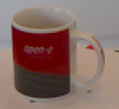
\includegraphics[width=\textwidth]{img/base/3.png}
            	\end{subfigure}
            	\begin{subfigure}{1.2cm}
            		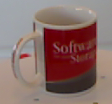
\includegraphics[width=\textwidth]{img/base/4.png}
            	\end{subfigure}
            \end{figure}

            \begin{itemize}
                \item 8 escenas
                \item Distintas instancias y categorías de objetos por escena
                \item Anotadas en RGB
            \end{itemize}

        \end{column}
    \end{columns}

    % \begin{itemize}
    %     \item objetos y escenas elegidos para seleccion de parametros
    %     \item seleccion/exploracion de parametros
    %     \item analisis sobre los metodos
    %     \item resultados por método y del sistema
    %     \item resultados del sistema con nuevos objetos
    % \end{itemize}
\end{frame}
%--- Next Frame ---%

\subsection{Selección de objetos para las pruebas}
\begin{frame}{Selección de objetos para las pruebas}
    % Decir por que se hicieron dos selecciones. La idea era "tunear" los métodos
    % y sus parámetros para algunos objetos representativos (3 categorías distintas)
    % y fijar los valores de parámetros que mejor se desempeñaran para los 3 casos

    % Una vez fijados estos valores, se usaron los otros 3 objetos y escenas donde
    % aparecen para corroborar la selección de parámetros realizada
    \begin{block}{Para la selección de parámetros}
        \begin{itemize}
            \item 3 objetos: taza blanca, gorra roja, bowl verde-agua
            \item 2 escenas: escritorio 1 y 2
        \end{itemize}
    \end{block}

    % Decir en estos casos por que se eligió cada objeto.
    % Taza: supuestamente buena para RGB por su textura y para depth por su forma
    % Lata: buena para depth por su forma, mala para RGB por su textura
    % Caja: Buena para RGB por su textura y mala para depth por ser plana
    \begin{block}{De control}
        \begin{itemize}
            \item 3 objetos: taza roja con dibujos, lata, caja de cereales
            \item 2 escenas: mesa grande y mesa pequeña
        \end{itemize}
    \end{block}
\end{frame}
%--- Next Frame ---%

\subsection{Métricas}
\begin{frame}[t]{Comparación de resultados vs. ground truth}
    IMAGEN DEL PDF DE PASCALLIN VOC METRIC QUE MUESTRA LO DE INTERSECCION / UNION
\end{frame}
%--- Next Frame ---%


\begin{frame}[t]{Selección del umbral de solapamiento}
    % Decir que es el accuracy: medida de que tan buenos son los resultados
    % reportados por el algoritmo.
    FORMULA DEL ACCURACY?\\
    GRAFICO DE UMBRAL VS ACCURACY\\
    % Comentar que umbral elegimos para el análisis posterior
\end{frame}
%--- Next Frame ---%

%%%%%%%%%%%%%%%%%%%%%%%%%%
%%%%%%%%%%%%%%%%%%%%%%%%%%
\section{Conclusiones y trabajo a futuro}
\begin{frame}{Conclusiones y trabajo a futuro}
    \begin{itemize}
        \item conclusiones
        \item mejoras a implementar
    \end{itemize}
\end{frame}
%--- Next Frame ---%


\end{document}


% TODO: Preguntar a Pachi si está bien esto: la detección/seguimiento en RGB no es facilmente utilizable para detectar objetos de una misma clase (no distinguir instancias sino clase de objetos) ya que en general dos objetos de la misma categoría pueden no compartir los mismos colores y esa información que pueden no compartir es justamente de la que se valen los metodos RGB para detectar/seguir un objeto. En template matching si se quieren detectar categorías se debería proveer al método de templates de todas las instancias que se pueden llegar a encontrar.
% En profundidad en cambio, como en general los objetos de la misma categoría comparten forma, se puede llegar a detectar un objeto dentro de una categoría para el cual no se haya entrenado el método de detección/seguimiento.
